\documentclass[conference]{IEEEtran}
\IEEEoverridecommandlockouts

\usepackage{amsmath,amssymb}
\usepackage{array}
\usepackage{booktabs}
\usepackage{cite}
\usepackage{graphicx}
\usepackage{tikz}
\usepackage{url}
\usetikzlibrary{arrows.meta,positioning}

\newcommand{\code}[1]{\texttt{#1}}

\begin{document}

\title{Modular and Auditable Clinical Extraction from Epilepsy Letters}

\author{\IEEEauthorblockN{Anonymous submission}}

\maketitle

\begin{abstract}
Clinical extraction systems need more than a single aggregate score: their
model, deterministic rules, repairs, evidence, scorer, and evaluation boundary
must remain separately inspectable. We evaluate a modular architecture on two
epilepsy-letter tasks: current seizure-frequency labeling on the Gan 2026
synthetic benchmark and broad epilepsy phenotyping on ExECTv2. For each task we
retain rules-only, LLM-only, and hybrid reference cells with executable source
closure and no-call replay. On the frozen Gan holdout, the operational
single-pass structured-event system reaches 364/450 Purist accuracy, while a
more complex multi-trace ceiling reaches 379/450. On ExECT dev140, the retained
deterministic, LLM-only, and hybrid references reach 0.3548 strict per-item F1,
0.7393 clinical-headline F1, and 0.9189 clinical-headline F1, respectively. A
bounded same-core full-200 aggregate comparison spans 0.8197--0.8566
clinical-headline F1 across Qwen 3.6 35B, GPT-4.1-mini, and DeepSeek chat.
Saved-output ablations show positive normalization contributions on both tasks,
while the evidence check is score-inert on those representative replays. The
contribution is a reproducible, stage-owned comparison with explicit claim
boundaries, not a claim of independent clinical validation, strict ExECT
benchmark reproduction, or a completed six-model result.
\end{abstract}

\begin{IEEEkeywords}
clinical information extraction, epilepsy, large language models, hybrid
systems, reproducibility, evidence provenance
\end{IEEEkeywords}

\section{Introduction}

Epilepsy letters combine temporal reasoning, clinical terminology, medication
regimens, investigation findings, and ambiguous current-versus-historical
statements. Large language models (LLMs) can broaden extraction, but a model
call can hide where a result came from. Deterministic systems are easier to
inspect, yet often fail on linguistic variation and long-range clinical
selection.

We study these approaches as explicit architecture families rather than as one
opaque pipeline. The same project contains a deep single-label task and a broad
multi-entity task. This makes it possible to ask which stages transfer, which
results depend on task-specific scoring, and where evidence is insufficient for
a stronger claim.

The paper contributes: (1) a retained two-task by three-family comparison with
exact replay closure; (2) explicit ownership of extraction, normalization,
projection, repair, evidence validation, and scoring; (3) frozen aggregate
evidence for the Gan operational-versus-ceiling trade-off and a three-model
ExECT transfer study; and (4) reproducibility controls that pin prompts,
scorers, splits, repair policies, runtime identifiers, dependencies, and
artifact hashes.

\section{Related Work}

ExECT demonstrated structured epilepsy extraction from unstructured clinic
letters and later work documented the corresponding annotation resource
\cite{fonferko2019exect,fonferko2024annotation}. Seizure-frequency extraction
has also been studied with machine-reading and pretrained-language-model
approaches \cite{xie2022seizure,abeysinghe2025leveraging}, while recent work
has explored fine-tuned LLMs and reproducible synthetic clinical letters
\cite{holgate2025fine,gan2026synthetic}. Our focus is complementary: pipeline
stages and evidence boundaries are part of the scientific object, and
rules-only, LLM-only, and hybrid forms are compared without collapsing their
different scoring and repair mechanisms.

\section{Methods}

\subsection{Tasks and Split Policy}

Gan 2026 asks for one current seizure-frequency label per synthetic letter
\cite{gan2026synthetic}. Validation750 is the row-inspectable development and
replay surface. Test450 is a locked holdout: only frozen aggregate results are
retained, and row-level holdout failures are not used for development.

ExECTv2 covers Diagnosis, SeizureFrequency, Prescription, and Investigations in
the primary comparison, with additional entities retained in the deterministic
all-nine reference \cite{fonferko2019exect,fonferko2024annotation}. Dev140 is
the row-inspectable development surface. Full200 combines dev140 with held-out
test60 and is reported only as a development-inclusive aggregate audit; it is
not an independent holdout.

\subsection{Architecture Families}

For each task, the retained manifest contains exactly one rules-only, LLM-only,
and hybrid cell. Rules-only cells use deterministic extraction, normalization,
projection, validation, and rendering without model calls. LLM-only cells
concentrate clinical extraction in one model program. The ExECT GEPA cell is a
negative development comparator, not the production control. Hybrid cells keep
model-owned clinical extraction distinct from deterministic selection,
normalization, evidence checks, and scoring. Gan uses one structured-event
pass; ExECT uses manifest-driven finding assembly with family-specific lenses.

\begin{figure}[tbp]
\centering
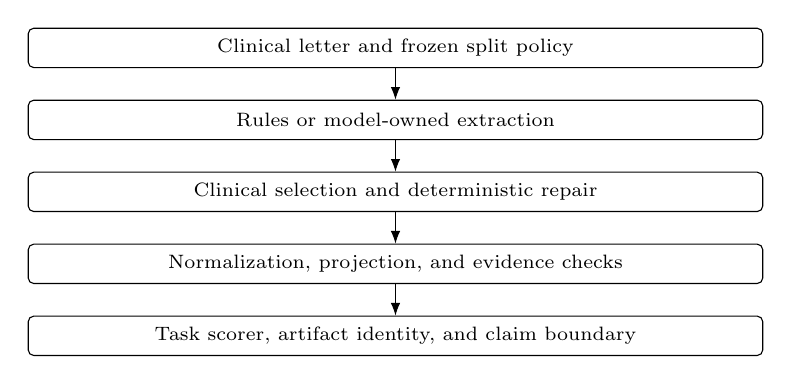
\begin{tikzpicture}[
  node distance=4mm,
  box/.style={draw,rounded corners=2pt,align=center,font=\scriptsize,
    text width=0.75\columnwidth,minimum height=5mm},
  arrow/.style={-{Latex[length=1.6mm]},line width=0.35pt}
]
\node[box] (input) {Clinical letter and frozen split policy};
\node[box,below=of input] (extract) {Rules or model-owned extraction};
\node[box,below=of extract] (clinical) {Clinical selection and deterministic repair};
\node[box,below=of clinical] (project) {Normalization, projection, and evidence checks};
\node[box,below=of project] (score) {Task scorer, artifact identity, and claim boundary};
\draw[arrow] (input) -- (extract);
\draw[arrow] (extract) -- (clinical);
\draw[arrow] (clinical) -- (project);
\draw[arrow] (project) -- (score);
\end{tikzpicture}
\caption{Stage-owned extraction spine. Ownership remains explicit even when a
stage is implemented by an LLM.}
\label{fig:spine}
\end{figure}

\subsection{Scoring, Repair, and Attribution}

Gan uses Purist and Pragmatic label scoring; Purist is the primary strict label
surface. ExECT's primary research-control surface is de-duplicated
\code{clinical\_headline} recovery across four families. Phrase, CUI,
evidence-valid, and full-attribute companions are reported separately.
\code{clinical\_headline} is not presented as reproduction of the published
strict ExECT benchmark.

Raw model selection, JSON or format repair, source-exact evidence repair,
deterministic semantic repair, projection, and final scoring are separate
stages. Model-specific transport or output-shape adapters do not become model
quality evidence. Semantic repairs retain a named deterministic owner and must
be ablated or otherwise tested before supporting a causal interpretation.

\subsection{Architecture Freeze}

The 14 July 2026 reduced-reference-architecture freeze pins the implementation
at commit \code{46562134}. Manifest v3 fingerprints the
dependency declaration and lock, prompt contracts, scorers, split manifests,
repair policies, model policy, split runbook, and CI workflow. A semantic
prompt, scorer, split, repair, runtime-route, or component-graph change requires
a new freeze and complete replay. The freeze does not itself authorize model
calls.

\section{Results}

\subsection{Retained Architecture Comparison}

Table~\ref{tab:reference-cells} is the minimum retained scientific comparison.
Scores are not compared across tasks because the datasets, outputs, and scorers
differ.

\begin{table}[!t]
\caption{Retained Two-Task by Three-Family Reference Cells}
\label{tab:reference-cells}
\centering
\scriptsize
\setlength{\tabcolsep}{2pt}
\begin{tabular}{@{}p{0.13\columnwidth}p{0.12\columnwidth}p{0.16\columnwidth}p{0.20\columnwidth}p{0.29\columnwidth}@{}}
\toprule
Task & Family & Split & Retained result & Role and boundary \\
\midrule
ExECTv2 & Rules only & dev140 & Strict item F1 0.3548 & Incomplete deterministic development reference. \\
ExECTv2 & LLM only & dev140 & Headline F1 0.7393 & GEPA negative development comparator. \\
ExECTv2 & Hybrid & dev140 & Headline F1 0.9189 & Current development performance control. \\
Gan 2026 & Rules only & validation750 & 697/750 Purist & Deterministic development comparator. \\
Gan 2026 & LLM only & validation750 & 581/750 Purist & Single-pass development comparator. \\
Gan 2026 & Hybrid & validation750 & 661/748 rendered Purist & Single-pass structured-event comparator. \\
\bottomrule
\end{tabular}
\end{table}

All six cells replay from current code and retained outputs without model calls.
The ExECT hybrid replay also returns evidence-valid F1 0.8913. Its current
benchmark/CUI companion is 0.4791 versus 0.4729 in the retained run artifact;
this companion-scorer drift is open and does not affect the reproduced 0.9189
headline result.

\subsection{Gan Frozen Holdout Evidence}

\begin{table}[tbp]
\caption{Gan Operational and Ceiling Evidence on Locked Test450}
\label{tab:gan-holdout}
\centering
\scriptsize
\begin{tabular}{lrl}
\toprule
System & Purist & Role \\
\midrule
Single structured-event pass & 364/450 & Operational close-off \\
V12 multi-trace reviewer & 379/450 & Complexity ceiling \\
\bottomrule
\end{tabular}
\end{table}

Both rows in Table~\ref{tab:gan-holdout} are frozen aggregate evidence. The
15-row quality difference does not yet support an efficiency conclusion. A
matched table of calls, tokens, cost, latency, hardware, and cache policy
remains open.

\subsection{ExECT Same-Core Model Evidence}

The retained model-transfer package holds the two-call no-SF-adjudicator
component graph fixed while changing the runtime model. Table~\ref{tab:model-swap}
is a full200 development-inclusive aggregate read; no test60 row-level analysis
is used.

\begin{table}[!t]
\caption{ExECT Same-Core Full200 Aggregate \code{clinical\_headline}}
\label{tab:model-swap}
\centering
\scriptsize
\resizebox{\columnwidth}{!}{%
\begin{tabular}{lrrrrrr}
\toprule
Model condition & Overall & Diagnosis & SF & Prescription & Investigations & Call/parse failures \\
\midrule
DeepSeek chat & 0.8566 & 0.8708 & 0.7602 & 0.8926 & 0.9091 & 0/1 \\
GPT-4.1-mini & 0.8356 & 0.8397 & 0.7525 & 0.8926 & 0.8563 & 0/0 \\
Qwen 3.6 35B repair v02 & 0.8197 & 0.8307 & 0.7020 & 0.8926 & 0.8503 & 0/0 \\
\bottomrule
\end{tabular}%
}
\end{table}

These runs support a bounded same-core transfer statement. They are not a
strict same-prompt panel: the retained GPT condition used temperature 0.3, and
Qwen used a compact prompt and output-contract repair. The requested six-model
comparison remains incomplete, with three missing runtime conditions requiring
predeclaration.

\subsection{Cross-Task Components and Reliability}

\begin{table}[tbp]
\caption{Saved-Output Component Ablation}
\label{tab:components}
\centering
\scriptsize
\begin{tabular}{lrr}
\toprule
Component & ExECT dev140 & Gan validation750 \\
\midrule
Normalization/dictionary & +0.0389 & +0.0293 \\
Evidence validation & 0.0000 & 0.0000 \\
\bottomrule
\end{tabular}
\end{table}

The zero score delta in Table~\ref{tab:components} does not show that evidence
validation is unnecessary. A filter may be essential on malformed or
hallucinated outputs even when all selected reference predictions already
satisfy it. Rejection and repair tests, not aggregate F1 alone, carry that part
of the evidence.

\begin{table}[!t]
\caption{Retained Reliability Evidence and Limits}
\label{tab:reliability}
\centering
\scriptsize
\begin{tabular}{@{}p{0.18\columnwidth}p{0.42\columnwidth}p{0.30\columnwidth}@{}}
\toprule
Subject & Retained result & Boundary \\
\midrule
ExECT evidence & Hybrid dev140 minimum exact evidence rate 1.0000 & Development reference. \\
ExECT calibration & Brier 0.2225; base-rate Brier 0.2340; ECE 0.0587 & Full200 aggregate internal scoring-rule result. \\
Gan grounding & Architecture-specific validation grounding packages retained & Metrics are not uniform across families. \\
Reproducibility & 1,153 tests, Ruff, mypy, hashes, split barriers, and six-cell replay pass on Python 3.11 & Engineering verification, not clinical validation. \\
\bottomrule
\end{tabular}
\end{table}

Model-reported confidence remains unused, and no low-burden review-routing
policy is promoted. The retained manifest does not include evidence for a
cross-task Wall-transfer claim.

\section{Discussion}

The strongest result is structural rather than universal. The reduced system
can reproduce six architecture cells while keeping component ownership and
evaluation boundaries explicit. Hybrid assembly is substantially stronger than
the retained ExECT rules-only and LLM-only development references on
\code{clinical\_headline}, but the three cells do not share a strict published
benchmark surface. Deterministic paper-comparable engineering remains open.

The model-transfer result shows that the component graph runs with three
qualitatively different runtime models. DeepSeek leads the retained full200
aggregate, while Qwen trails most clearly on SeizureFrequency. Because runtime
conditions are asymmetric and the panel is only three of six, this is evidence
of bounded portability rather than a universal model-agnostic claim.

The cross-task ablation suggests that normalization is useful in both tasks.
The evidence gate's zero F1 delta illustrates why clinical pipeline evidence
cannot be reduced to aggregate score changes: rejection, provenance, and repair
behavior need direct contract tests.

\section{Limitations}

Gan test450 is frozen aggregate evidence and cannot support row-level tuning.
ExECT full200 includes dev140 and is not an independent holdout.
\code{clinical\_headline} is a clinical-recovery surface, not the published
strict benchmark. The ExECT benchmark/CUI companion has small current-code
replay drift. The model panel is three of six and uses asymmetric runtime
conditions. Model-reported confidence and low-burden review routing are not
validated. Annotation-quality findings are internally adjudicated; unqualified
clinical validity would require independent domain review. The current retained
evidence does not support an ExECT Wall-transfer claim.

\section{Conclusion}

A small, frozen, stage-owned clinical extraction system can preserve both
performance evidence and the provenance needed to interpret it. The retained
results support a two-task rules/LLM/hybrid comparison, a bounded Gan
operational-versus-ceiling result, and a three-model ExECT same-core study. They
do not yet support strict ExECT benchmark reproduction, a six-model conclusion,
or independent clinical validation. Those boundaries are part of the result,
not footnotes to it.

\section*{Reproducibility Statement}

The machine-readable retained-evidence manifest records the six reference
cells, selected artifacts and hashes, policy fingerprints, and no-call replay
expectations. The synchronized Markdown manuscript and this IEEE source use
only evidence retained by that manifest and claim strength permitted by the
paper-provenance canon.

\begin{thebibliography}{00}
\bibitem{fonferko2019exect} B. Fonferko-Shadrach, A. S. Lacey, A. Roberts,
S. Thompson, D. V. Ford, R. A. Lyons, M. I. Rees, and W. O. Pickrell, ``Using
natural language processing to extract structured epilepsy data from
unstructured clinic letters: development and validation of the ExECT
(extraction of epilepsy clinical text) system,'' \emph{BMJ Open}, vol. 9,
no. 4, e023232, 2019, doi: 10.1136/bmjopen-2018-023232.

\bibitem{fonferko2024annotation} B. Fonferko-Shadrach \emph{et al.},
``Annotation of epilepsy clinic letters for natural language processing,''
\emph{Journal of Biomedical Semantics}, vol. 15, no. 17, 2024, doi:
10.1186/s13326-024-00316-z.

\bibitem{xie2022seizure} K. Xie \emph{et al.}, ``Extracting seizure frequency
from epilepsy clinic notes: a machine reading approach to natural language
processing,'' \emph{Journal of the American Medical Informatics Association},
vol. 29, no. 5, pp. 873--881, 2022, doi: 10.1093/jamia/ocac018.

\bibitem{abeysinghe2025leveraging} R. Abeysinghe, S. Tao, S. D. Lhatoo,
G.-Q. Zhang, and L. Cui, ``Leveraging pretrained language models for seizure
frequency extraction from epilepsy evaluation reports,'' \emph{npj Digital
Medicine}, 2025, doi: 10.1038/s41746-025-01592-4.

\bibitem{holgate2025fine} B. Holgate, J. Davies, S. Fang, J. Winston,
J. Teo, and M. Richardson, ``Fine-tuning LLMs to extract epilepsy seizure
frequency data from health records,'' in \emph{Proc. 24th Workshop on
Biomedical Language Processing}, Vienna, Austria, 2025, pp. 44--55, doi:
10.18653/v1/2025.bionlp-1.5.

\bibitem{gan2026synthetic} Y. Gan, S. H. Barlow, B. Holgate, J. Davies,
J. T. Teo, J. S. Winston, and M. P. Richardson, ``Reproducible synthetic
clinical letters for seizure frequency information extraction,'' arXiv:
2603.11407, 2026.
\end{thebibliography}

\end{document}
